\chapter{Modeling Preparation for Research Tasks}
\label{chap:verification-tensile-sc}
As the primary goal of this research is to develop a database of elastic-plastic finite element models and results for flat plates in bending, the programs and techniques used to create that database can be validated against existing tension cases.
These techniques are first applied to models used for EPRI \hone calculations, then to a group of models demonstrating load separation, and finally to two models from the existing TASC program leading to an interpolated result for an intermediate material.

\section{EPRI \hone Verification}
\label{sec:h1-verification}

The finite element method used in the EPRI report \citep{epri1981} was extended to fully-plastic \J solutions for three-dimensional geometries in \citet{mcclung1999}.
ABAQUS was used for the elastic-plastic analysis using an incremental plasticity model.
\Cref{fig:geometries} shows the models examined for \(n=5, 10, \textnormal{ and } 15\).
Once values for \Jpl were calculated, \hone values comparable to the EPRI graphs were calculated as
\begin{align}
\hone &= \frac{\Jpl}{\alpha \sigma_0 \epsilon_0 t \left( \frac{\sigma}{\sigma_0}\right)^{n+1}} \label{eq:h1mcclung}
\end{align}
using a Ramberg-Osgood power-law material model.
\citet{lei2004} ran both elastic and elastic-plastic models for the same geometries with \(n=5\) and \(n=10\).
\citet{quillen2005} ran both elastic-plastic and fully-plastic models with various mesh densities, element types, and material models.
Each of Quillen's Abaqus models had some anomalies in the \hone values compared to McClung and Lei at the free surface, the symmetry plane, and at the third node from the free surface.
Values at each of these positions was higher than the trend exhibited by neighboring points.
Some models displayed small discrepancies, others were quite large.
At the time, no reason was identified for the anomalies. \Cref{fig:model3_n10_2005,fig:model5_n5_2005} show two such sets of discrepancies.

\begin{figure}[tbp]
    \centering
    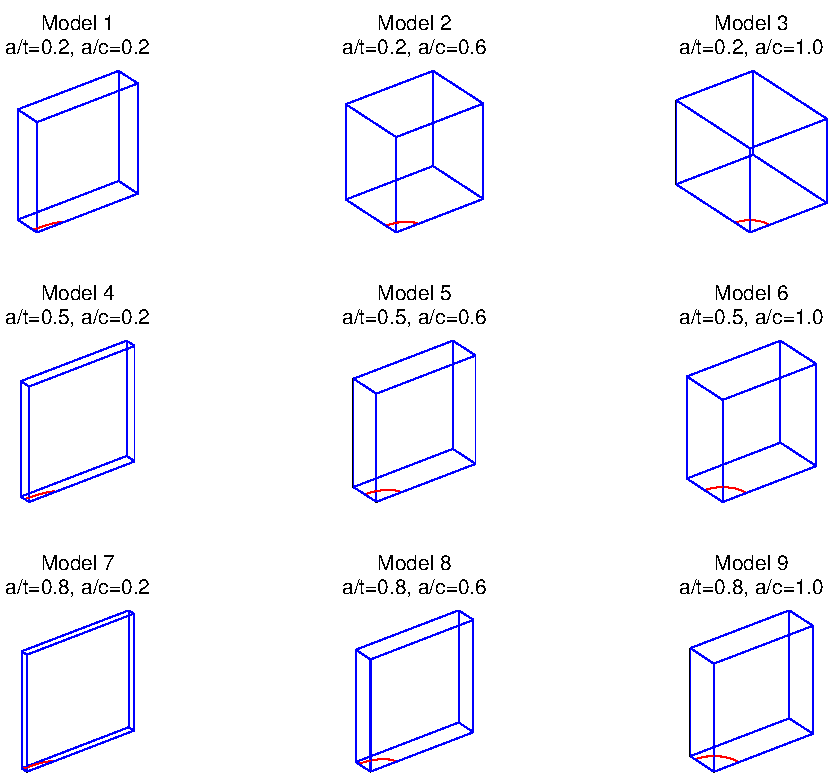
\includegraphics[width=0.8\columnwidth]{geometries}
    \caption{McClung et al. model geometry \label{fig:geometries}}
\end{figure}

\begin{figure}[tbp]
  \centering
  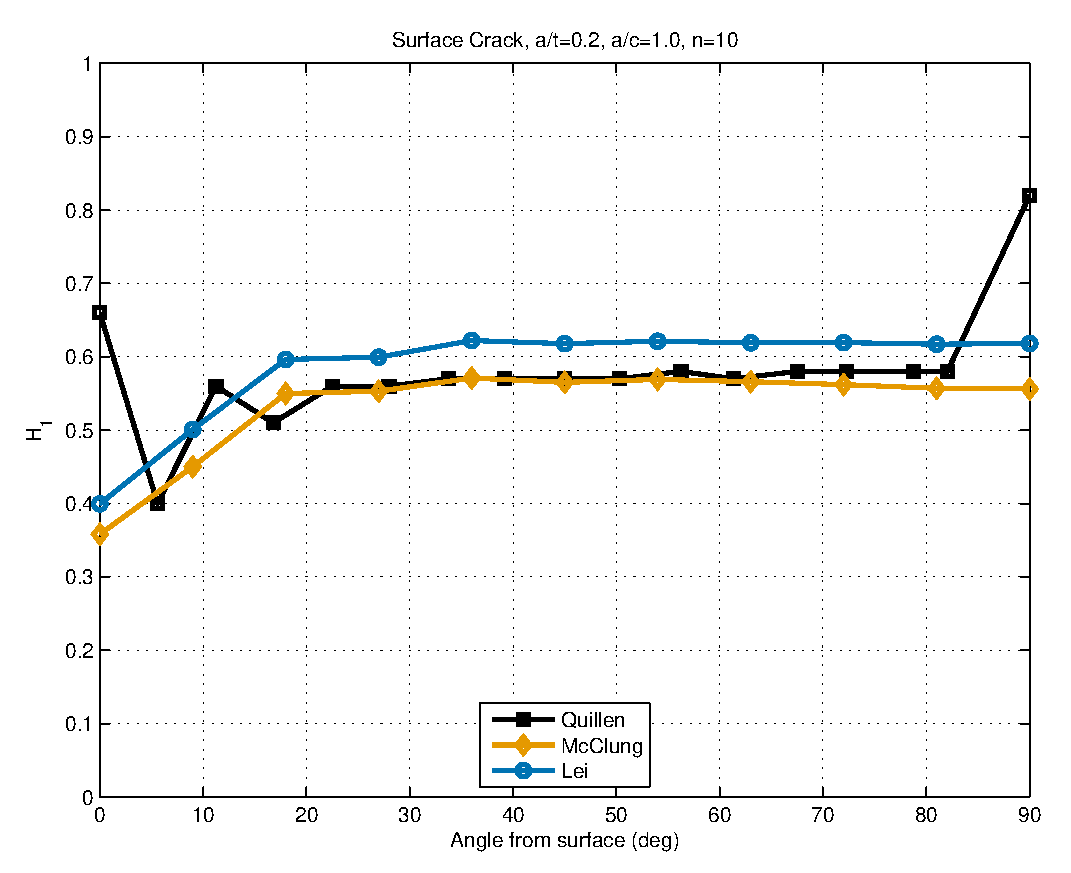
\includegraphics[width=0.6\columnwidth]{model3_n10}
  \caption[\hone comparison between \citeauthor{quillen2005}, McClung et al., and Lei, model 3, \(n=10\)]{\hone comparison between \citet{quillen2005}, McClung et al., and Lei, model 3, \(n=10\) \label{fig:model3_n10_2005}}
\end{figure}
\begin{figure}
  \centering
  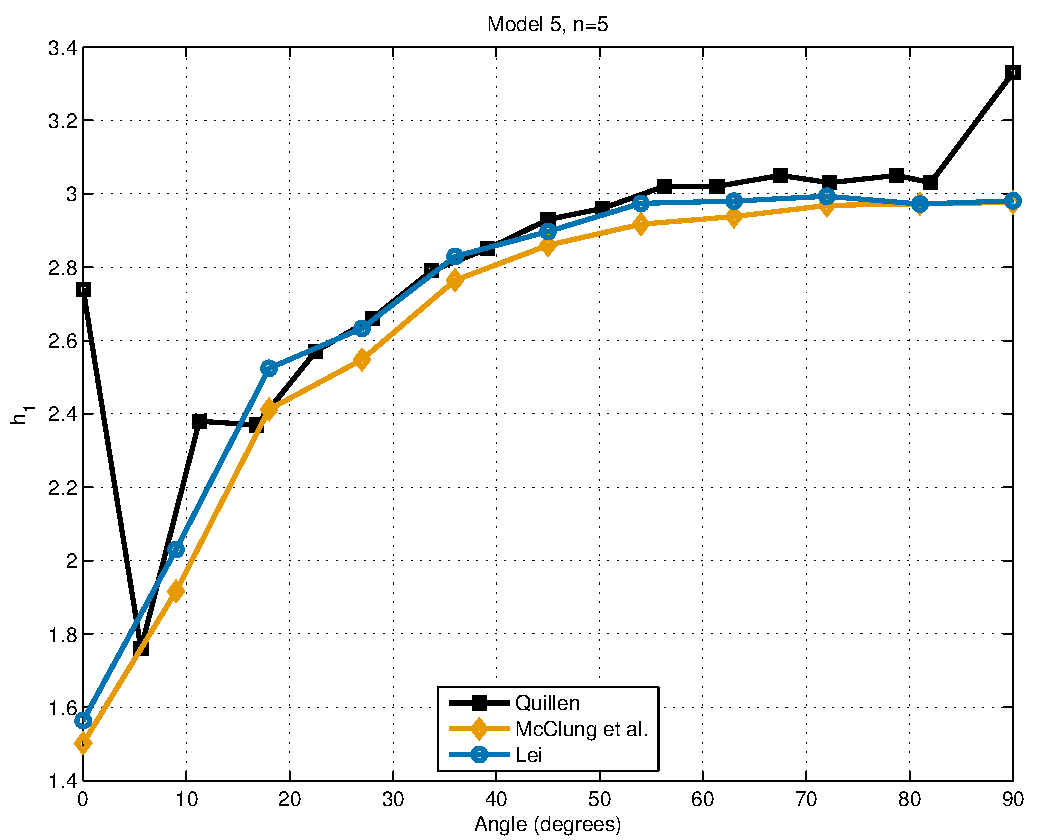
\includegraphics[width=0.6\columnwidth]{model5_n5}
  \caption[\hone comparison between \citeauthor{quillen2005}, McClung et al., and Lei, model 5, \(n=5\)]{\hone comparison between \citet{quillen2005}, McClung et al., and Lei, model 5, \(n=5\) \label{fig:model5_n5_2005}}
\end{figure}

\Cref{chap:app-quillen-rework} shows more detail on the development of some early Python programs used to create and analyze the plate and crack geometries shown in \Cref{fig:geometries}.
For each of the nine geometries, finite element models with varying numbers of elements were created.
For each finite element mesh, one linear elastic and three Ramberg-Osgood elastic-plastic models were analyzed, and \J values were stored in the Abaqus ODB.
Finally, \hone values were calculated from the \J values to test for convergence and verification against earlier models.
A total of 144 models were analyzed, including 36 elastic models (nine geometries by four mesh densities) and 108 elastic-plastic models (nine geometries by four mesh densities by three Ramberg-Osgood hardening exponents).
Solving all the models required approximately 43 hours on one quad-core AMD Opteron compute cluster node, and created \SI{103}{\giga\byte} of output data. Extracting \hone data from the ODB files took only 7 minutes.
Mesh convergence for one model is shown in \Cref{fig:mesh-convergence}, and convergence on the ratio of \Jpl:\Jel is shown in \Cref{fig:j-convergence}.
Note that the mesh convergence is not due simply to creating smaller elements along the crack front.
As shown in \Cref{fig:model1-3-meshes}, the number of elements along the crack front only increases from 21 to 25.
Adding additional elements outside the crack region has an effect on the \J and \hone values calculated, indicating that this model set needs further development.
However, all three anomalous \hone results in \citet{quillen2005} have been eliminated, as shown in \Cref{fig:model1}.
The root cause of the anomalies (errors in the original files generated by FEACrack, possible unrecorded modifications to the files, bugs corrected in Abaqus, etc.) is still unknown.

  \begin{figure}[tbp]
    \centering
    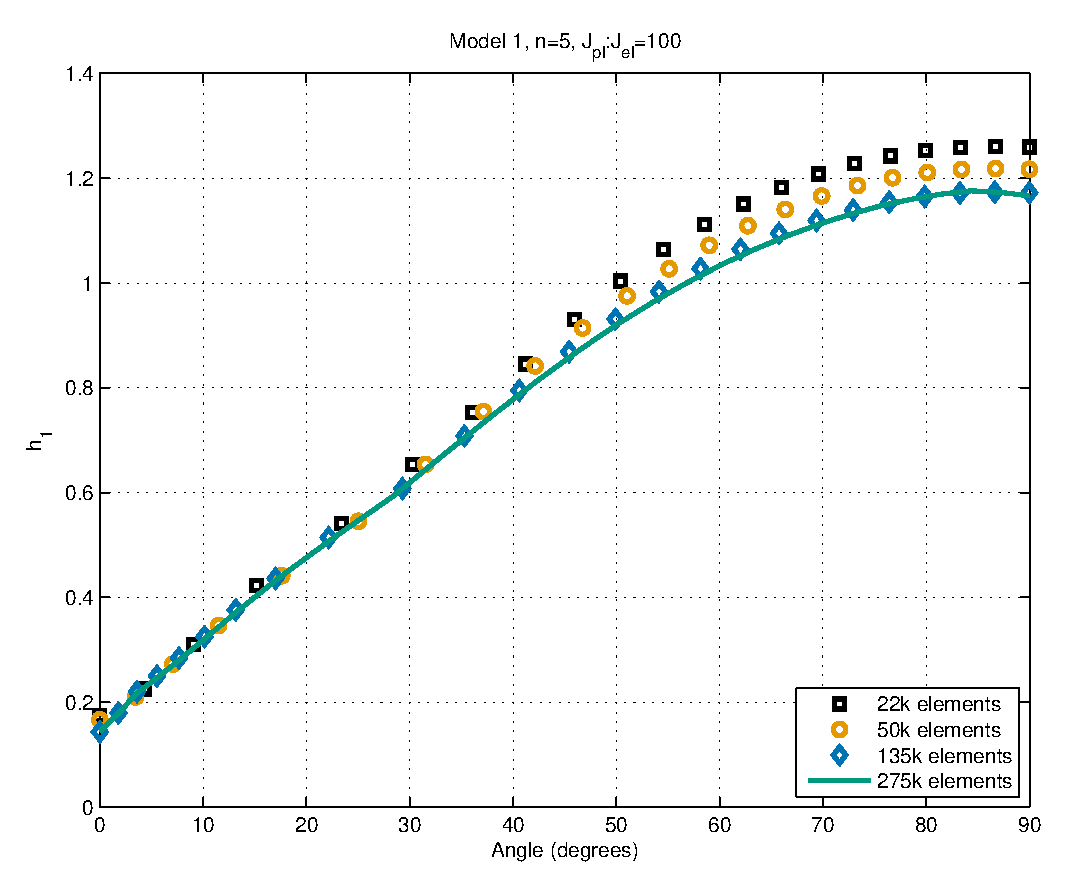
\includegraphics[width=0.6\columnwidth]{model1_n5_mesh_convergence}
    \caption{McClung et al. model 1 mesh convergence\label{fig:mesh-convergence}}
  \end{figure}
  \begin{figure}[tbp]
    \centering
    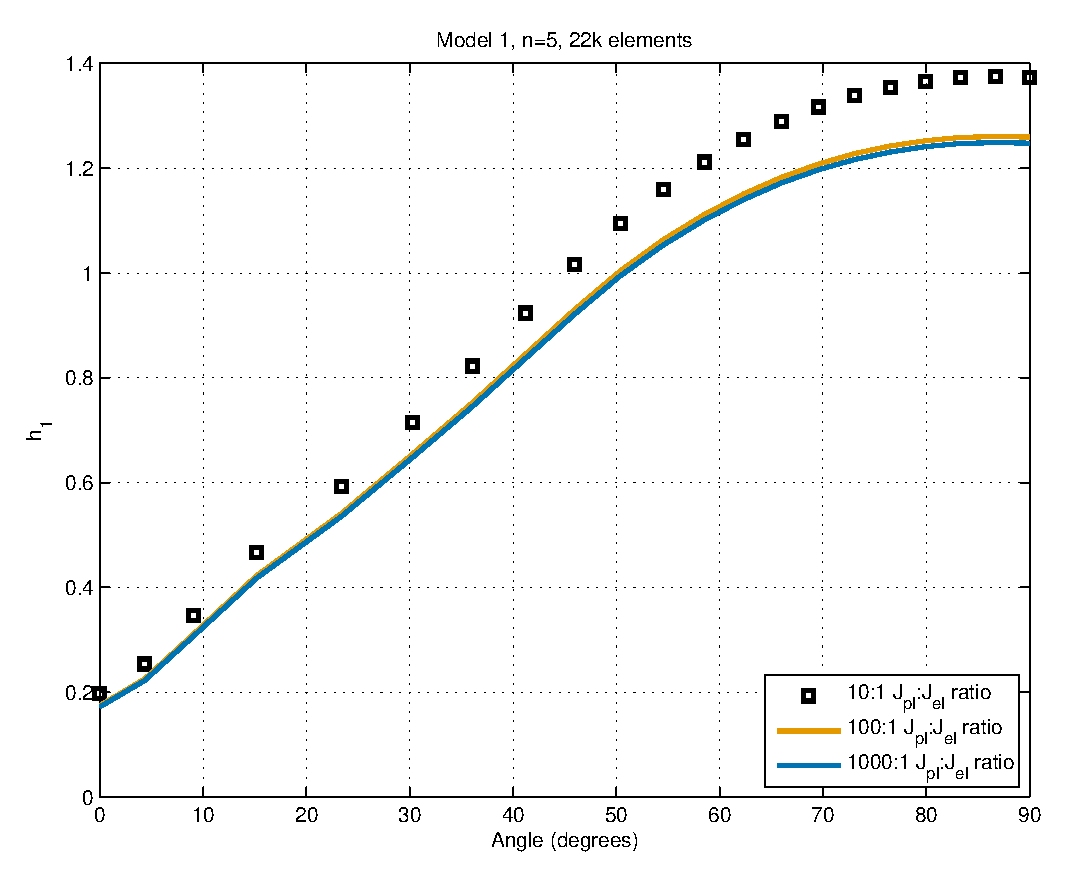
\includegraphics[width=0.6\columnwidth]{model1_n5_J_convergence}
    \caption{McClung et al. model 1 \J ratio convergence\label{fig:j-convergence}}
  \end{figure}

  \begin{figure}[tbp]
    \centering
    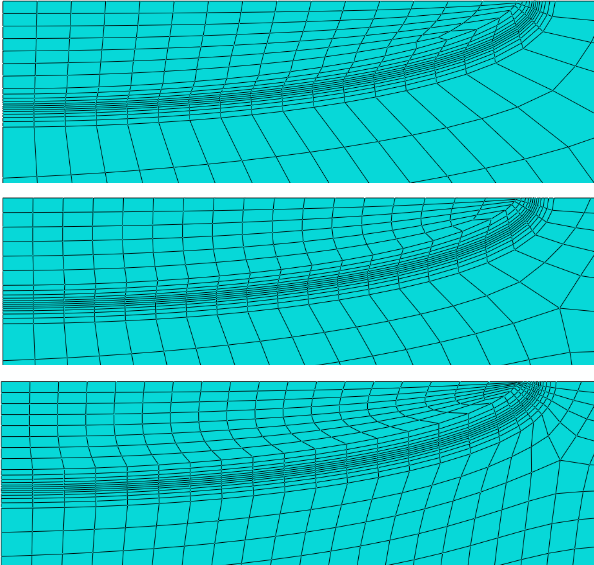
\includegraphics[width=0.6\columnwidth]{model1-3-meshes}
    \caption{McClung et al. model 1 crack front mesh detail\label{fig:model1-3-meshes}}
  \end{figure}
  \begin{figure}[tbp]
    \centering
    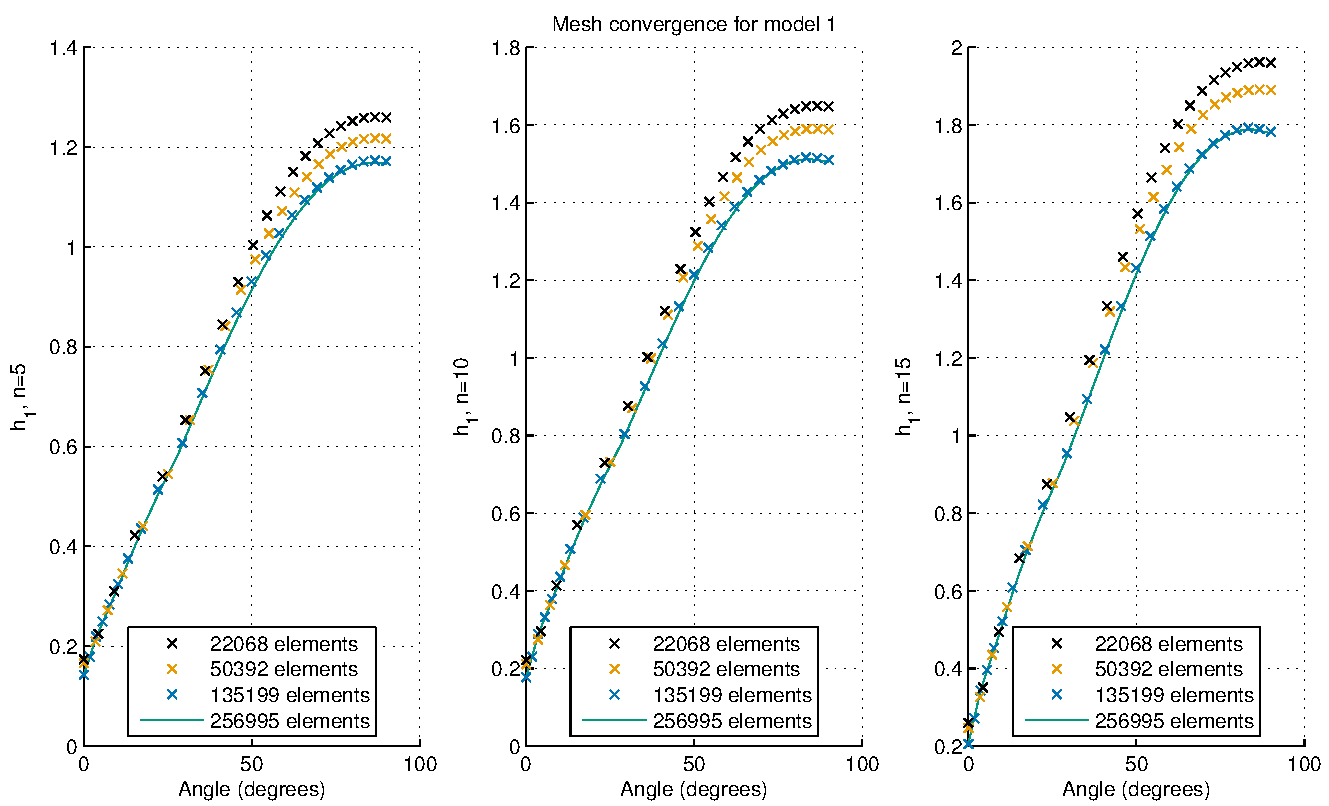
\includegraphics[width=\columnwidth]{h1_model1}
    \caption{\hone comparison between McClung et al., Lei, and Renfro, model 1 \label{fig:model1}}
  \end{figure}

\FloatBarrier
\section{Load Separation Verifications}
\label{sec:loadsepverification}

A brief check of the results of the \citet{sharobeamlandes1993} load separation results for surface cracks in tension was performed.
The six data points used in \Cref{fig:bet_Sij_original} were correlated back to specific crack sizes, and the most similar surface crack models from the TASC geometry set, \((\frac{a}{c}, \frac{a}{t}) = (0.6, 0.2), (0.6, 0.4), (0.6, 0.6), (1.0, 0.4)\), were adapted to include tension boundary conditions.
Remote tensile stress versus total CMOD and plastic CMOD for the four crack shapes is shown in \Cref{fig:stress-cmod-tension}.
The separation parameters \Sij using data from \((\frac{a}{c}, \frac{a}{t}) = (0.6, 0.6)\) as the reference curve is shown in \Cref{fig:sij_cmodpl}, and is limited to CMOD values greater than 0.01 in order to emphasize the regions with significant plastic behavior.
Finally, the correlation between \Sij and the effective uncracked ligament length for the original work from \citeauthor{sharobeamlandes1993} and for the current study are shown in \Cref{fig:sij_bet}, where both plots show relatively linear trends.
\begin{figure}[tbp]
\centering
\begin{minipage}{0.45\textwidth}
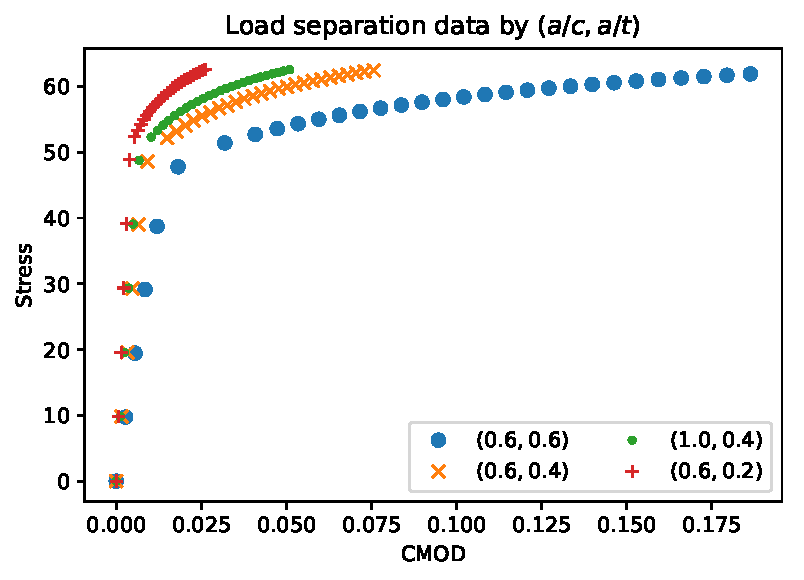
\includegraphics[width=\textwidth]{loadsep-stress-cmod-tension}
\subcaption{\label{fig:stress-cmod} Tensile stress versus CMOD}
\end{minipage}
\begin{minipage}{0.45\textwidth}
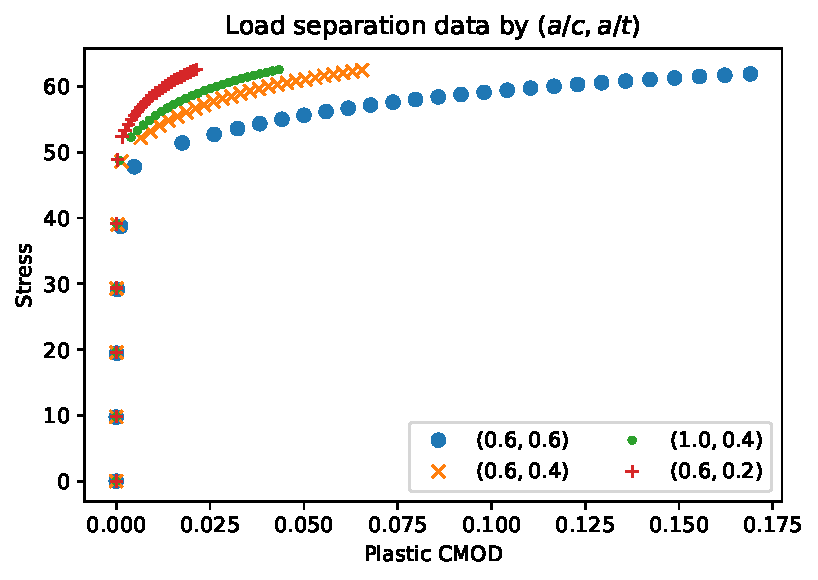
\includegraphics[width=\textwidth]{loadsep-stress-cmodpl-tension}
\subcaption{\label{fig:stress-cmodpl} Tensile stress versus plastic CMOD}
\end{minipage}
\caption{\label{fig:stress-cmod-tension} Initial load separation applied to surface cracks in tension}
\end{figure}
\begin{figure}[tbp]
\centering
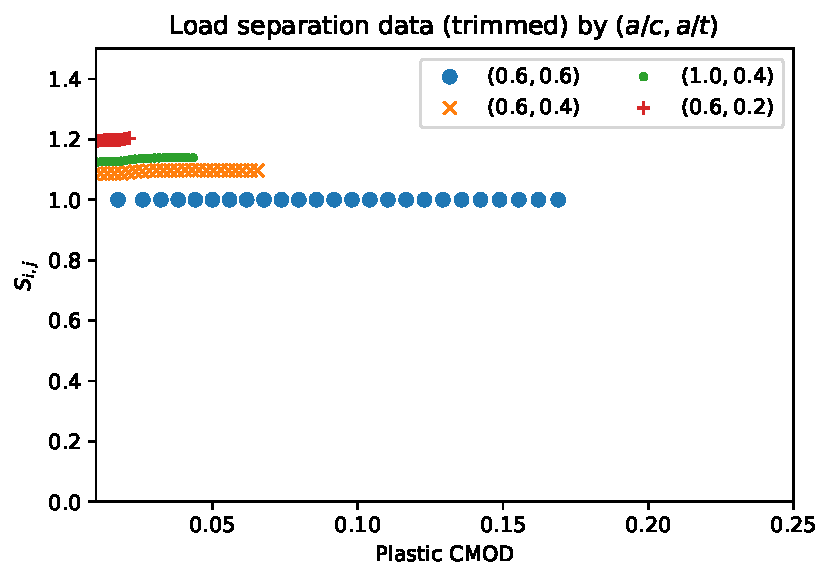
\includegraphics[width=0.8\textwidth]{cmodpl_Sij_tension}
\caption{\label{fig:sij_cmodpl} Separation parameter values versus plastic CMOD}
\end{figure}
\begin{figure}[tbp]
\centering
\begin{minipage}{0.45\textwidth}
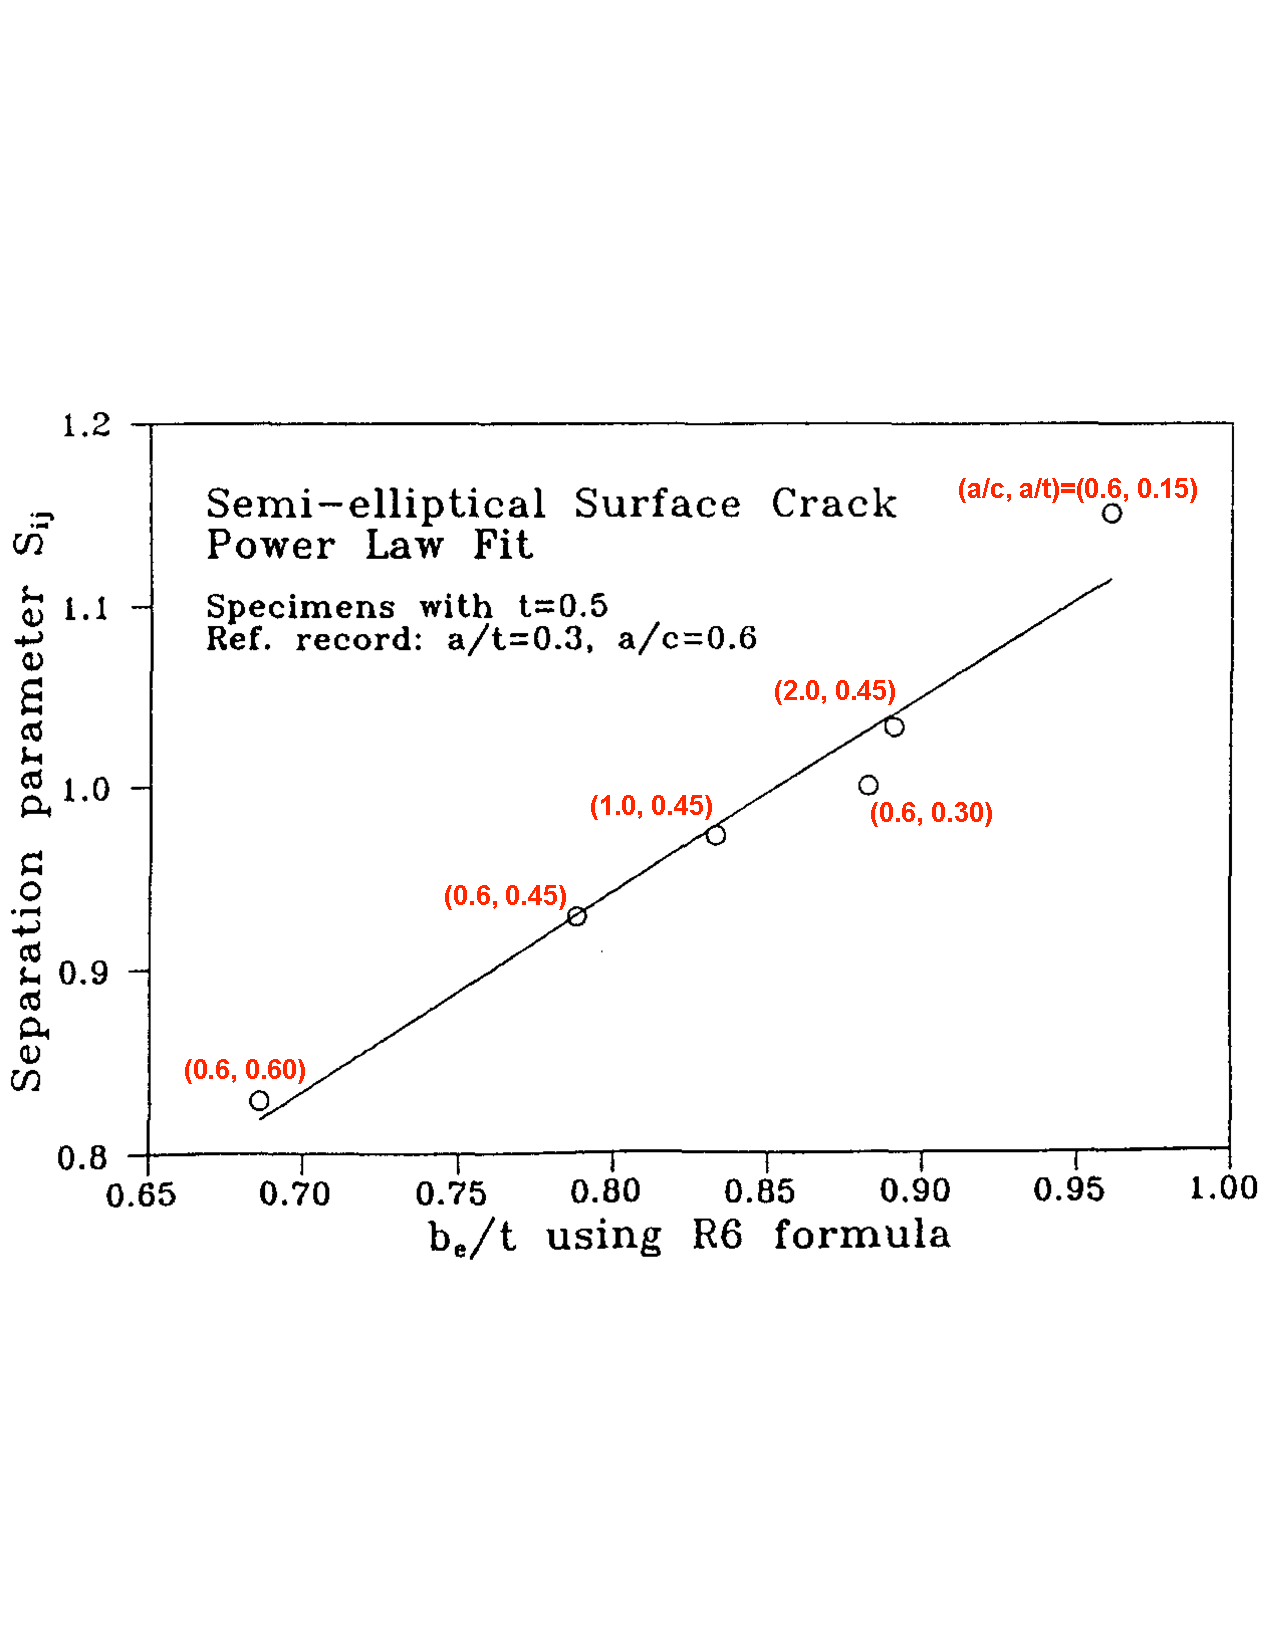
\includegraphics[width=\textwidth]{load-sep-tension-sl-2}
\subcaption{\label{fig:load-sep-tension-sl} Annotated from \cite{sharobeamlandes1993}}
\end{minipage}
\begin{minipage}{0.45\textwidth}
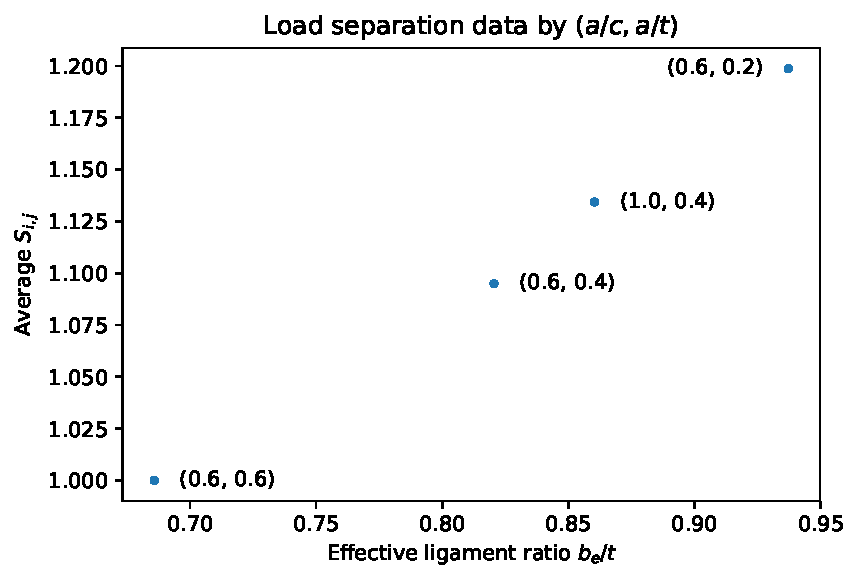
\includegraphics[width=\textwidth]{bet_Sij_tension}
\subcaption{\label{fig:load-sep-tension-mwr} From current work}
\end{minipage}
\caption{\label{fig:sij_bet} Separation parameter values versus effective uncracked ligament length}
\end{figure}

\FloatBarrier

\section{Verification of Two TASC Cases}
\label{sec:verification-tasc}

The next chapter will show the development of a set of modeling tools to study surface cracks in flat plates, using FEACrack, Python, and WARP3D.
This section details the first use of these tools in verifying two tension models from \citeauthor{allenwells2014} (\citeyear{allenwells2014}), and then to solve an intermediate case, demonstrating the limits of the interpolation methodology.
Details of the algorithms used in the Python programs are given in \Crefrange{sec:preprocess}{sec:postprocess}.

\subsection{Identified Gaps in Interpolation Data}

\citeauthor{allenwells2014} built a set of 600 finite element models of surface cracks in tension, covering all combinations of
\begin{align*}
\frac{a}{t} &= 0.2, 0.4, 0.6, 0.8 & \frac{E}{\Sys} &= 100, 200, 300, 500, 700, 1000 \\
\frac{a}{c} &= 0.2, 0.4, 0.6, 0.8, 1.0 & n &= 3, 4, 6, 10, 20.
\end{align*}
Results for a set of models with \(\frac{a}{t}=0.6\) and \(n=6\) are shown in \Cref{fig:aspect-ratio-gap,fig:modulus-gap}.
The first figure shows a large gap between the results for cases \(\frac{a}{c}=0.2\) and \(\frac{a}{c}=0.4\), and the second figure shows a similar gap between the results for cases \(\frac{E}{\Sys}=100\) and \(\frac{E}{\Sys}=200\).
In each figure, normalized CMOD values for the more extreme case nearly double at comparable normalized stress levels, and the normalized \J values for the more extreme case are reduced by almost half at identical normalized CMOD levels.
As the authors use the solved models in a linear interpolation method, they identified a potential need for additional models with \(\frac{a}{c}=0.3\) and \(\frac{E}{\Sys}=150\), since there is no guarantee that the cracked plates exhibit linear behavior over such a wide range of results.
\begin{figure}[tbp]
\centering
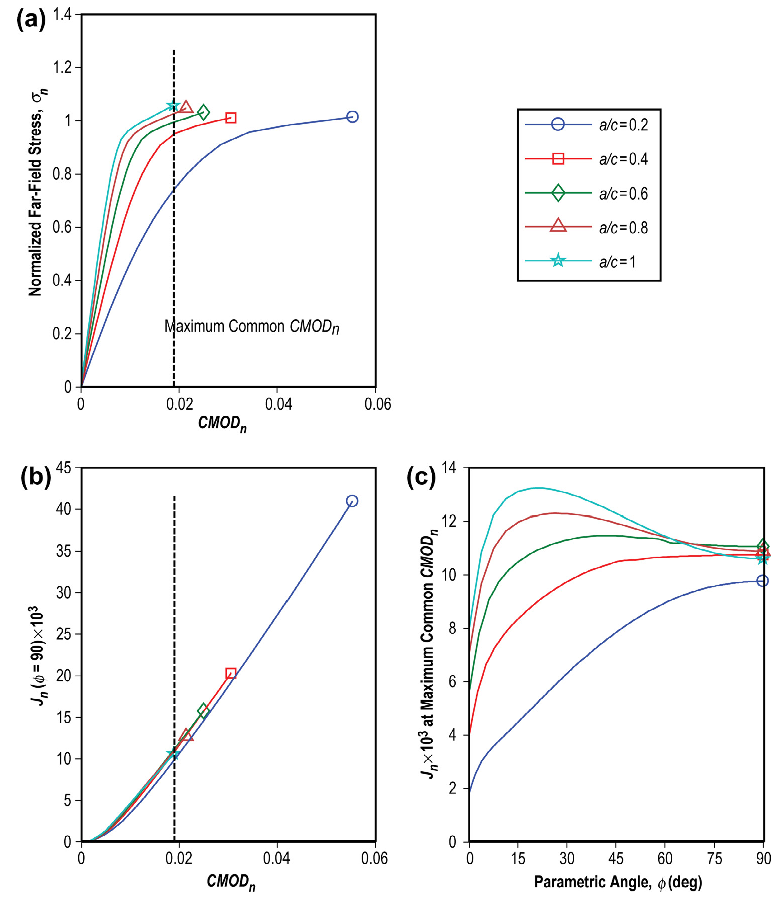
\includegraphics[width=0.7\columnwidth]{aspect-ratio-gap}
\caption[Gap in results for very wide aspect ratios]{\label{fig:aspect-ratio-gap} Gap in results for very wide aspect ratios \citep{allenwells2014}}
\end{figure}
\begin{figure}[tbp]
\centering
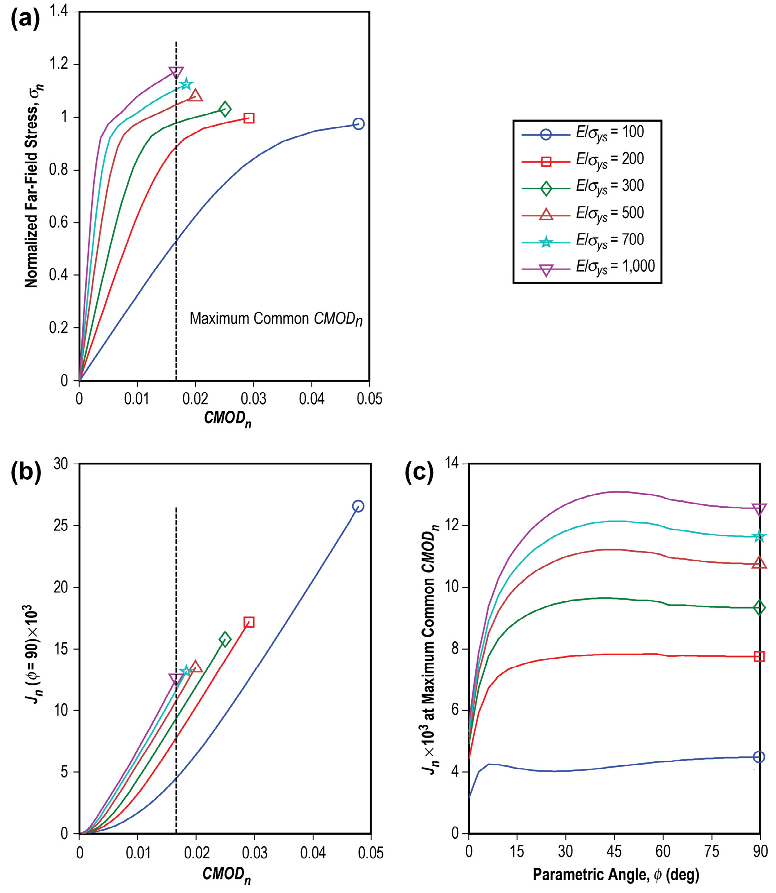
\includegraphics[width=0.7\columnwidth]{modulus-gap}
\caption[Gap in results for very low elastic modulus values]{\label{fig:modulus-gap} Gap in results for very low elastic modulus values \citep{allenwells2014}}
\end{figure}

\Cref{chap:app-verification-allen-wells} details the use of FEACrack \citep{feacrack} and WARP3D \citep{warp3d} to replicate the published results for the cases
\begin{align*}
\frac{a}{t} &= 0.6 & \frac{E}{\Sys} &= 100 \text{ and } 200\\
\frac{a}{c} &= 0.6 & n &= 6
\end{align*}
and the remainder of this section will show the results of a purpose-built model for \(\frac{E}{\Sys} = 150\) compared to an interpolated model using results from \(\frac{E}{\Sys}=100\) and \(\frac{E}{\Sys}=200\).

\subsection{Applying Procedure to New Material Model (\(\frac{E}{\Sys} = 150\))}

After modifying the \(\frac{E}{\Sys} = 200\) model from \Cref{chap:app-verification-allen-wells} to use \(E = 150\) and leaving the normalized remote displacement at 0.0550, the new material model was solved.
As seen in \Cref{fig:e150_1}, the remote displacement was not high enough to place the model into the plastic regime, so the remote displacement was increased to 0.080.
The result of the new displacement is shown in \Cref{fig:e150_2}, and has clearly reached the plastic regime.
Later models used the secant method to adjust boundary conditions to meet a desired amount of plastic behavior, and reached a CMOD of roughly 0.03.
\begin{figure}[tbp]
\centering
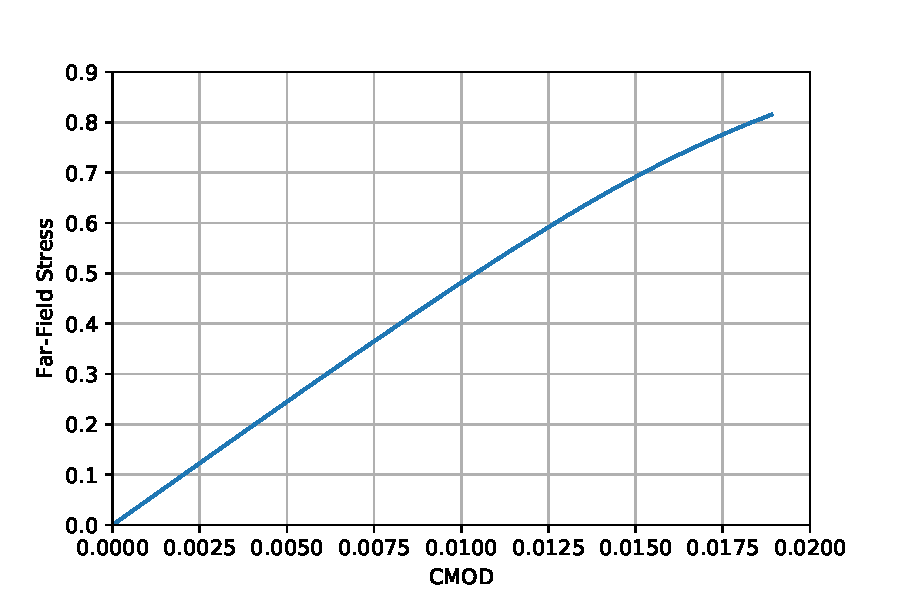
\includegraphics[width=0.8\columnwidth]{e150_1}
\caption{\label{fig:e150_1} First attempt at new material model}
\end{figure}
\begin{figure}[tbp]
\centering
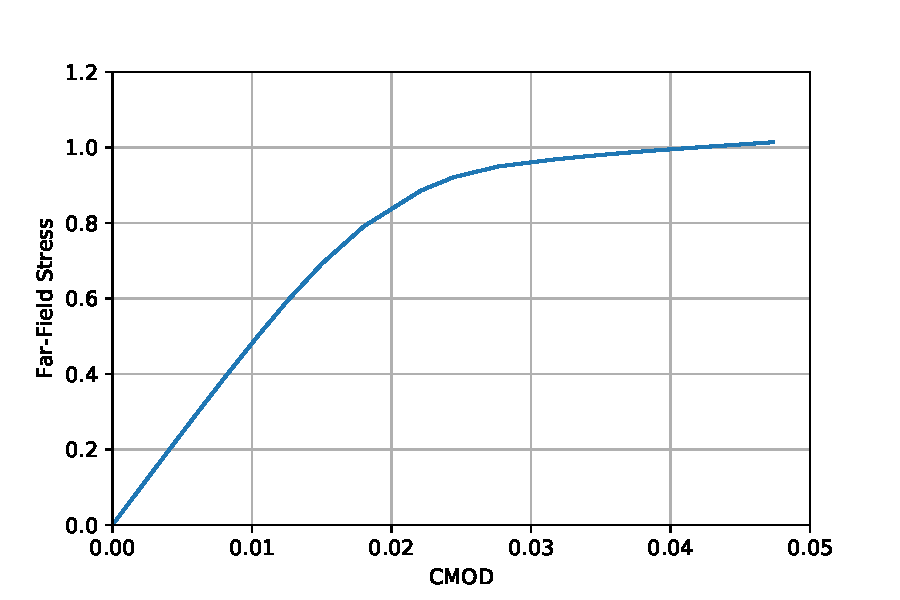
\includegraphics[width=0.8\columnwidth]{e150_2}
\caption{\label{fig:e150_2} Second attempt at new material model}
\end{figure}

Finally, by comparing the \(\frac{E}{\Sys} = 150\) FEA results to the interpolated TASC result from \Cref{fig:tasc_interp_outputs}, the FEA results are slightly more compliant in the elastic regime, and a sharper transition to the plastic regime at higher stress levels.
The two results differ by 5\% or less, as shown in \Cref{fig:e100_150_200_verification}.
\begin{figure}[tbp]
\centering
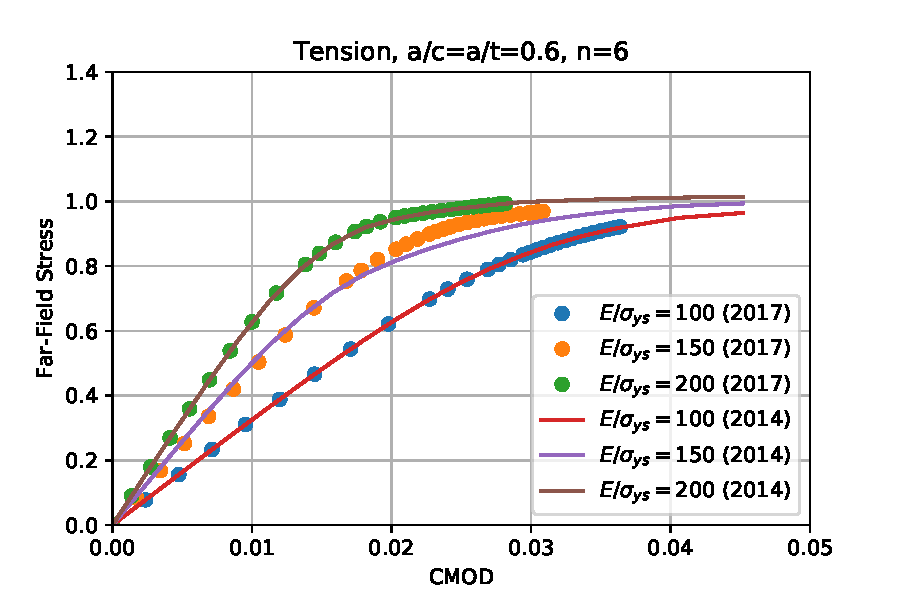
\includegraphics[width=0.8\columnwidth]{e100_150_200_verification}
\caption{\label{fig:e100_150_200_verification} Comparison of normalized FEA results, interpolated result, and TASC raw data}
\end{figure}

\subsection{Plotting CMOD, \J and \(\phi\)}

The final data to extract from the FEA results are values for the \J integral at each load increment. \J is a function of both load and position along the crack front, measured by the angle \(\phi\) from the free surface of the plate.
An example of the \J-\(\phi\)-CMOD relationship from \cite{allenwells2014} is shown in \Cref{fig:j-phi-cmod-paa}, while a comparable relationship from the current models is shown in \Cref{fig:j-phi-cmod-mwr}.
In both cases, higher CMOD values correlate with higher \J values, and \J values at a given CMOD are higher deep in the crack than at the free surface.
\begin{figure}[bp]
\centering
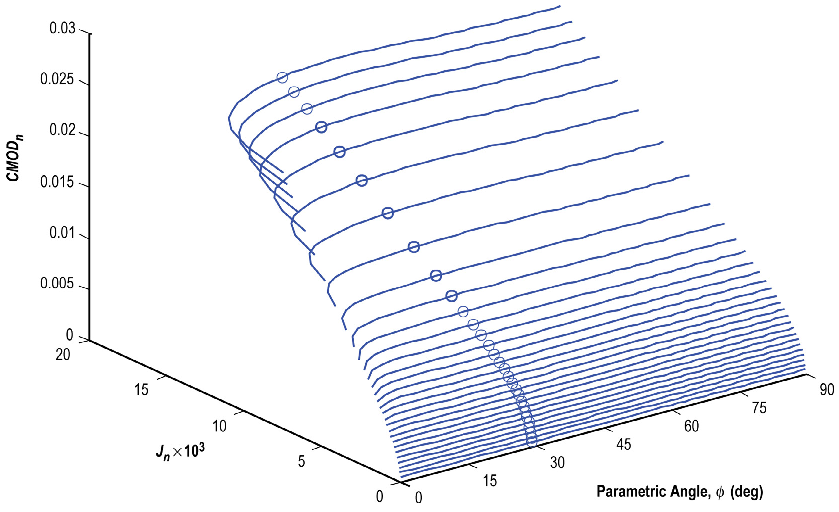
\includegraphics[width=0.8\columnwidth]{j-phi-cmod-paa}
\caption[Example relationship between \(\J(\phi)\) and CMOD from TASC]{\label{fig:j-phi-cmod-paa} Example relationship between \(\J(\phi)\) and CMOD from TASC\citep{allenwells2014}}
\end{figure}

\begin{figure}[tbp]
\centering
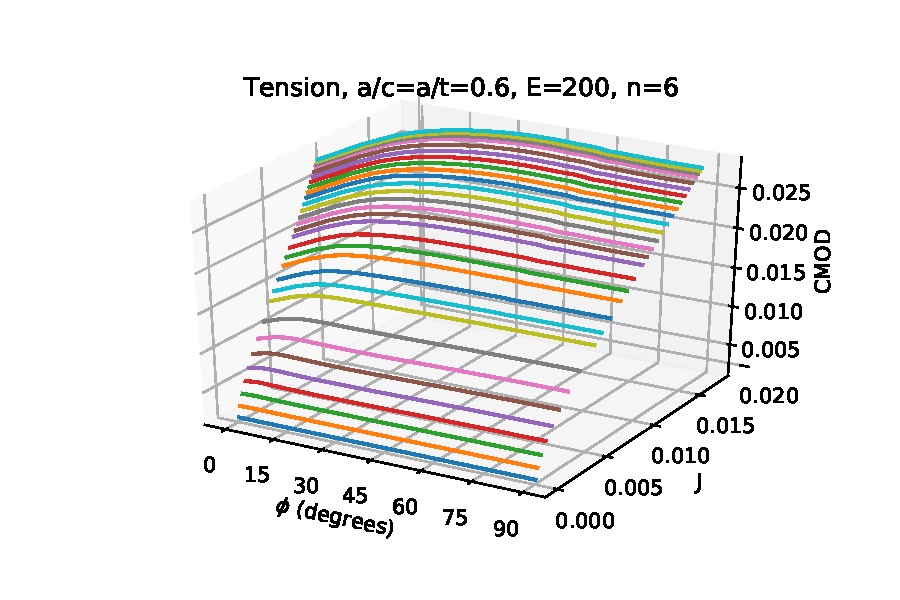
\includegraphics[width=0.8\columnwidth]{j-phi-cmod-mwr}
\caption{\label{fig:j-phi-cmod-mwr} Example relationship between \(\J(\phi)\) and CMOD}
\end{figure}

